\documentclass[../main.tex]{subfiles}
\begin{document}

\section{Stand der Technik}

\subsection{Additive Fertigung}

Additive Fertigung, unabhängig von dem Werkstoff, ist ein Bereich im dem viel
geforscht und innoviert wird. In fast jedem Industriebereich wird versucht ein
bestehendes Design oder Modell zu optimieren und verbessern. \cite{newMethod}
Sei es hinsichtlich Qualität oder Kosteneffizienz. Additive Fertigung bietet bei 
dieser Optimierung viele Vorteile gegenüber spanenden Fertigungsverfahren, da 
Additive Fertigung einen höheren Grad der Gestaltungsfreiheit bietet. 
Additive Fertigung ist eine Ressource den Benutzern ermöglicht komplexe 
Bauteilgeometrien zu erstellen ohne die Limitierung von konventionellen spanenden 
Herstellungsverfahren, wie hoher Materialverschleiß oder die Notwendigkeit von 
spezialisierten Werkzeugen. \cite{Vafadar.2021} 

Außerdem können mit additiver Fertigung Stückzahlen drastisch reduziert werden.
Werkstücke können bei Bedarf gefertigt werden, was die Notwendigkeit für Lagerstätten
größtenteils eliminiert. Zusätzlich können die Teile genau dort herstellt werden, wo 
sie benötigt werden, was Lieferketten und Wartezeiten verkürzt.

Verschiedene Werkstoffe können mit additiver Fertigung (AF) benutzt werden, darunter
sind Polymeren, Metalle und Keramik. Metalle haben vor allem in den letzten Jahren 
an Relevanz gewonnen. Zusätzlich zu den schon genannten Vorteile von AF, 
bietet Metall als Werkstoff noch mehr Nutzen in der Industrie. Gegenüber Kunststoffen
produziert Metall weniger Abfall und kann eine höhere Qualität gewährleisten.
Zusätzlich dazu kommen die offensichtlichen Vorteile von Metall gegenüber Polymeren: 
höhere Hitzebeständigkeit und eine stabilere Grundstruktur, was sie weniger anfällig 
für Verformungen macht.

Aufgrund dieser Vorteile wird AF in vielen Industriebereichen genutzt. Die folgende
Sektion zeigt einige Fälle in denen AF erfolgreich benutzt wurde.

\subsubsection*{Automobil-Branche}

Eine der führenden Branchen in der AF-Entwicklung ist die Automobil-Branche. 
Durch den Herstellungsprozess
könne Teile gefertigt werden die leichter, belastbarer und sicherer sind. Die 
einfache Anpassbarkeit für geringen Entwicklungszeiten und Kosten. 
BWM zum Beispiel benutzt für den i8 Roadster viele AF gefertigte Teile.
Darunter die Befestigung für das Soft-Top, die 44 \% leichter als das Spritzgussteil
ist, und dennoch 10 Mal steifer. \cite{Vafadar.2021} 
Die Führung für das Fenster wurde auch additiv gefertigt, durch den "HP Multi Jet Fusion" 
konnten 100 Teile in 24 Stunden gefertigt werden. Selbst teile des Zylinderkopfs für den 
S58 Motor sind auch additiv gefertigt. \cite{Anusci.2019}

Auch bei älteren Fahrzeugen kann additive Fertigung Verwendung finden.
Gerade bei älteren Fabrikaten sind Ersatzteile häufig nicht mehr vom 
Erstzulieferer zu beschaffen oder mit konventionellen Herstellungsmethoden
wirtschaftlich herzustellen.
Hier wurde zum Beispiel die rechte 
Kotflügelhalterung für ein Matra 530 aus 1973 erfolgreich hergestellt, nachdem auch nach längerem suchen
kein Originalteil gefunden wurde \cite{AMExpo365.03.06.2024}. Zusätzlich war
bei diesem Beispiel die Herausforderung, das keine digitale Version des
Bauteils existiert hat. Zuerst musste das also als Grundlage für die
additive Fertigung erzeugt werden. Dies bringt mich zu meinem nächsten Punkt:

\subsection{Reverse Engineering}

Reverse Engineering beschreibt dem Prozess aus einem bestehenden Produkt 
oder Objekt ein digitales Abbild zu erzeuge \cite{Helle.2021}.
Dabei sind meistens wenig oder keine technischen Details über das Objekt
verfügbar. Gründe dafür können sein das der ursprüngliche Hersteller die 
Baupläne nicht veröffentlicht hat, um nicht der Konkurrenz in die Hände
zu spielen. Auch denkbar ist ein militärischer Hintergrund, hier werden
die Baupläne aus offensichtlichen Gründen auch nicht öffentlich zugänglich
sein. Das ist zum Beispiel in der Luftfahrtbranche, unter anderem bei dem
Hersteller Boeing, der Fall. 
Selbst wenn Baupläne vorhanden sind kann es trotzdem notwendig sein 
Reverse Engineering zu betreiben, denn das tatsächliche Produkt kann von
den Bauplänen abweichen, zum Beispiel durch jahrelange Benutzung oder
Toleranzen in der Herstellung. Wenn technische Details vorhanden sind,
können diese aber im Reverse Engineering Prozess verwendet werden.
Hier wird dieser Prozess beschrieben wie mithilfe einer Kombination von
originalen Bauplänen und 3D Laser Scanning ein möglichst genaues digitales
Abbild erzeugt werden kann \cite{Monchinger.2021}.
In dem Paper wird der Ansatz des Reverse Engineering genutzt um
bestehende Bauteile passgenau erweitern zu können. Konkret geht es um die
Entwicklung einer Methodik um automatisiert Laser-Scans und originale Baupläne
zusammenzufügen um ein möglichst detailgetreues Abbild der realen Struktur zu
erzeugen. Dieses Abbild wird dann benutzt, um die bestehende Struktur zu 
erweitern und auf ihr aufzubauen. Das wird am Beispiel eines Flugzeugs 
demonstriert, erst wird der Innenraum gescannt und mit dem originalen Plänen
abgeglichen, dann ein 3D Objekt erstellt. Mithilfe dieses 3D-Objekts können 
dann passgenaue Bauteile herstellt werden, die es ermöglichen ein ehemaliges 
Passierflugzeug zu einer Frachtmaschine umzubauen.
Wie schon erwähnt wird zur erfolgreichen Weiterbearbeitung ein möglichst 
genaues digitales Abbild benötigt.
Ist dies nicht der Fall müssen nicht passende Teile erneut hergestellt werden, 
was die Material- und Personalkosten deutlich erhöht. Es ist also im 
wirtschaftlichen Interesse beim ersten Schritt, dem Erstellen der digitalen 
Version, sehr genau und gewissenhaft vorzugehen um ein möglichst genaues Ergebnis
zu erzielen. Um eine digitale Version zu erstellen, existieren verschiedene Verfahren.
Auf einige werde ich im nächsten Abschnitt genauer eingehen.


\subsection{3D Rekonstruktion}

Digitale Abbildungen von Flächen, Objekten oder sogar Körperteilen wurden in den
letzten Jahren mehr und mehr benutzt. Anwendungen sind zum Beispiel in der
geometrischem Dokumentation, Inspektion, Navigation, Visualisierung und 
Objekterkennung zu finden \cite{Verykokou.2023}. Je nach Anwendungsfall wird eine
bestimmte Akkuranz
der Daten erwartet, im Medizinischen Bereich sind die Ansprüche natürlich ganz 
andere als zum Beispiel in der Dokumentierung von ganzen Gebirgszügen.
Aus diesem Grund existieren auch verschiedene Herangehensweisen und Technologien  
zur 3D-Rekonstruktion.
3D Rekonstruktion-Technologien können in 2 Kategorien eingeteilt werden,
die bildbasierte Verfahren und die Verfahren die auf Scandaten 
beruhen. \cite{Verykokou.2023}
Beide Verfahren können auch kombiniert werden. 
Bei bildbasierten Verfahren, auch Photogrammetrie genannt, wird das 3D Objekt aus
mehreren 2D Bildern erstellt, umso mehr Bilder vorhanden sind umso besser kann das
3D Objekt rekonstruiert werden. Um das 3D Objekt zu erstellen werden in 
allen Bildern gemeinsame Punkte gesucht und dann mit der bekannten Kameraposition, 
die relative Position des Punktes im 3D Objekt ermittelt. Figur x zeigt dies 
anschaulich.
Vorteile der Photogrammetrie sind die relativ einfache Aufnahme der Daten, schon
ein Smartphone mit Kamera kann ausreichend hochauflösende Bilder aufnehmen, um 
eine 3D-Rekonstruktion zu ermöglichen. Des Weiteren sind viele Softwarelösungen
auch kostenlos vorhanden um automatisiert 3D Objekte, auch ohne viele 
Vorkenntnisse, zu erzeugen.
Gründe sich gegen die Photogrammetrie zu entscheiden ist die doch limitierte 
Auflösung beziehungsweise steigt der Arbeitsaufwand drastisch umso akkurater
das Endergebnis sein soll. Auf der anderen Seite glänzt die Photogrammetrie aber 
bei 3D Rekonstruktionen im großen Stil wie zum Beispiel bei Gebäuden, Stadtteilen
oder Geografischen Strukturen.

Die Akkuranz bei der Photogrammetrie kann dabei, bei großen Objekten, in der 
Größenordnung Zentimeter liegen \cite{10004712}

\begin{figure}[h]
    \centering
    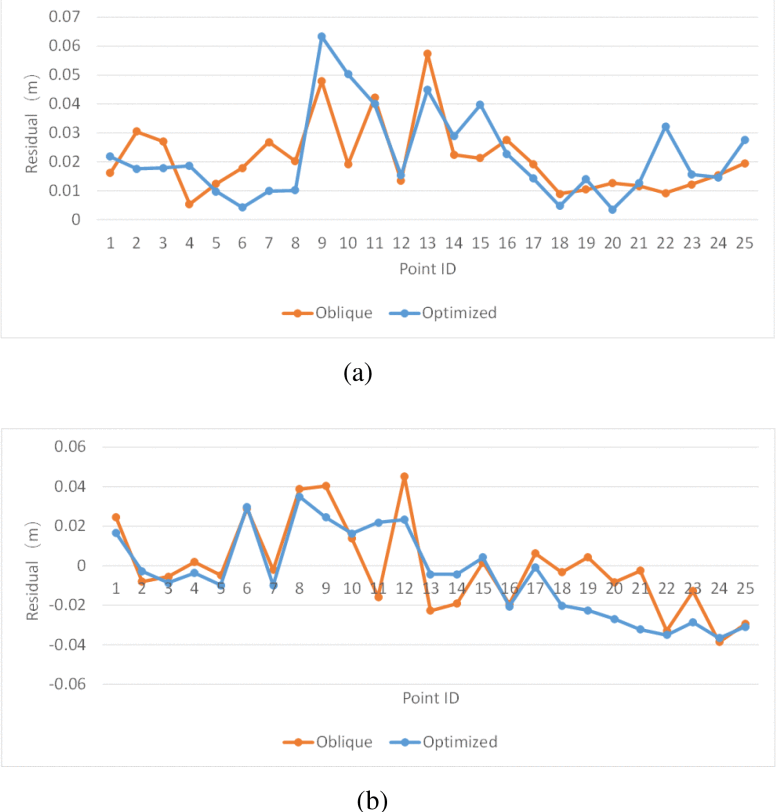
\includegraphics[height=150pt]{images/photogammatry_accurancy.PNG}
    \caption{Accurancy Photogrammetry}
    \label{fig:photogammatryAccuracy}
\end{figure}


Bei kleinen Objekten, wenn eine hinreichende Akkuranz gefordert ist sollte man 
deswegen zum 2. Verfahren greifen. Hier sind die Ursprungsdaten schon 
dreidimensional mit einem Scanner aufgenommen. Um an diese Daten zu kommen, 
misst ein Scanner, meistens mithilfe von Lichtstrahlen, den Abstand zu einem 
Punkt auf dem zu rekonstruierenden Objekt. Dann wird entweder das Objekt oder 
der Scanner bewegt, um so möglichst viele Scan punkte aufzunehmen.
Je mehr Punkte vorliegen, desto genauer wird das Ergebnis, allerdings steigt
auch die vorhandene Datenmenge mit, ab einem Punkt kann der verfügbare 
Speicher ein limitierender Faktor sein. Außerdem steigt die Rechenzeit auch mit
der Datenmenge, je nach anschließendem Verfahren sogar exponentiell.

Nachteile von diesem Verfahren sind die hohen initialen Kosten eines Scanners 
und der begrenzte Messbereich. 


\end{document}